\documentclass[12pt]{article}
\usepackage[utf8]{inputenc}

\title{Sprawozdanie\\z projektu Wirtualna Kamera\\„Spolens"}
\author{Daniel Sporysz}
\date{28.03.2020}

\usepackage{natbib}
\usepackage{graphicx}
\usepackage[polish]{babel}
\usepackage{polski}
\usepackage{indentfirst}
\usepackage[margin=1in]{geometry}
\usepackage{verbatim}

\usepackage{listings} % Required for inserting code snippets

\begin{document}

\makeatletter
\newcommand{\linia}{\rule{\linewidth}{0.4mm}}
\renewcommand{\maketitle}{\begin{titlepage}
    \begin{center}\LARGE
    Politechnika Warszawska\\Wydział Elektryczny
    \end{center}
    \vspace{4cm}
    \noindent
    \begin{center}
      \LARGE \textsc{\@title}
         \end{center}
    \vspace{4cm}
    \begin{flushright}
    \begin{minipage}{5cm}
    \textit{Autor:}\\
    \normalsize \textsc{\@author} \par
    \end{minipage}
     \end{flushright}
    \vspace*{\stretch{6}}
    \begin{center}
    \vspace*{\fill}
    \@date
    \end{center}
  \end{titlepage}%
}
\makeatother

\maketitle
\newpage

\tableofcontents
\newpage

\section{Opis projektu}
„Spolens" to program do generowania widoku na trójwymiarową przestrzeń, widzianego z wirtualnej kamery, której ruchami i parametrami sterować można za pomocą klawiatury.
Konfiguracja położenia i koloru elementów w przestrzeni jest wczytywana z pliku przy starcie programu.

\section{Wymagania techniczne}
Do uruchomienia należy zainstalować Python 3.8, a następnie zainstalować moduł Pyglet do Python.

\section{Funkcjonalność programu}

\subsection{Interfejs graficzny}
Po wywołaniu programu, tworzone jest nowe okno w którym wyświetlany jest widok z wirtualnej kamery, klawisze sterujące oraz wartości parametrów.

\begin{center}
    \noindent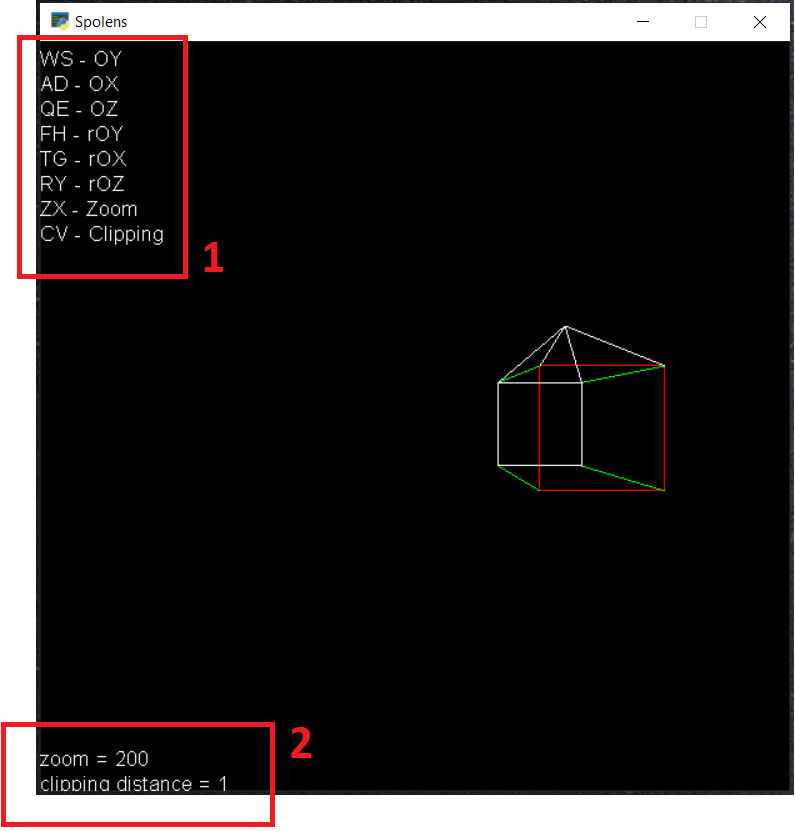
\includegraphics[scale=0.5]{spolens ui.png}
\end{center}

W zaznaczeniu @1 wypisana jest lista klawiszy sterujących wraz z nazwą akcji, która jest z nimi związana.

Zaznaczenie @2 wskazuje na aktualne wartości parametrow.

\newpage
\subsection{Translacja}
Przesunięciem kontrolujemy za pomocą klawiszy:
\begin{itemize}
    \item A/D w osi OY,
    \item W/S w osi OX,
    \item Q/E w osi OZ.
\end{itemize}

\begin{center}
    \noindent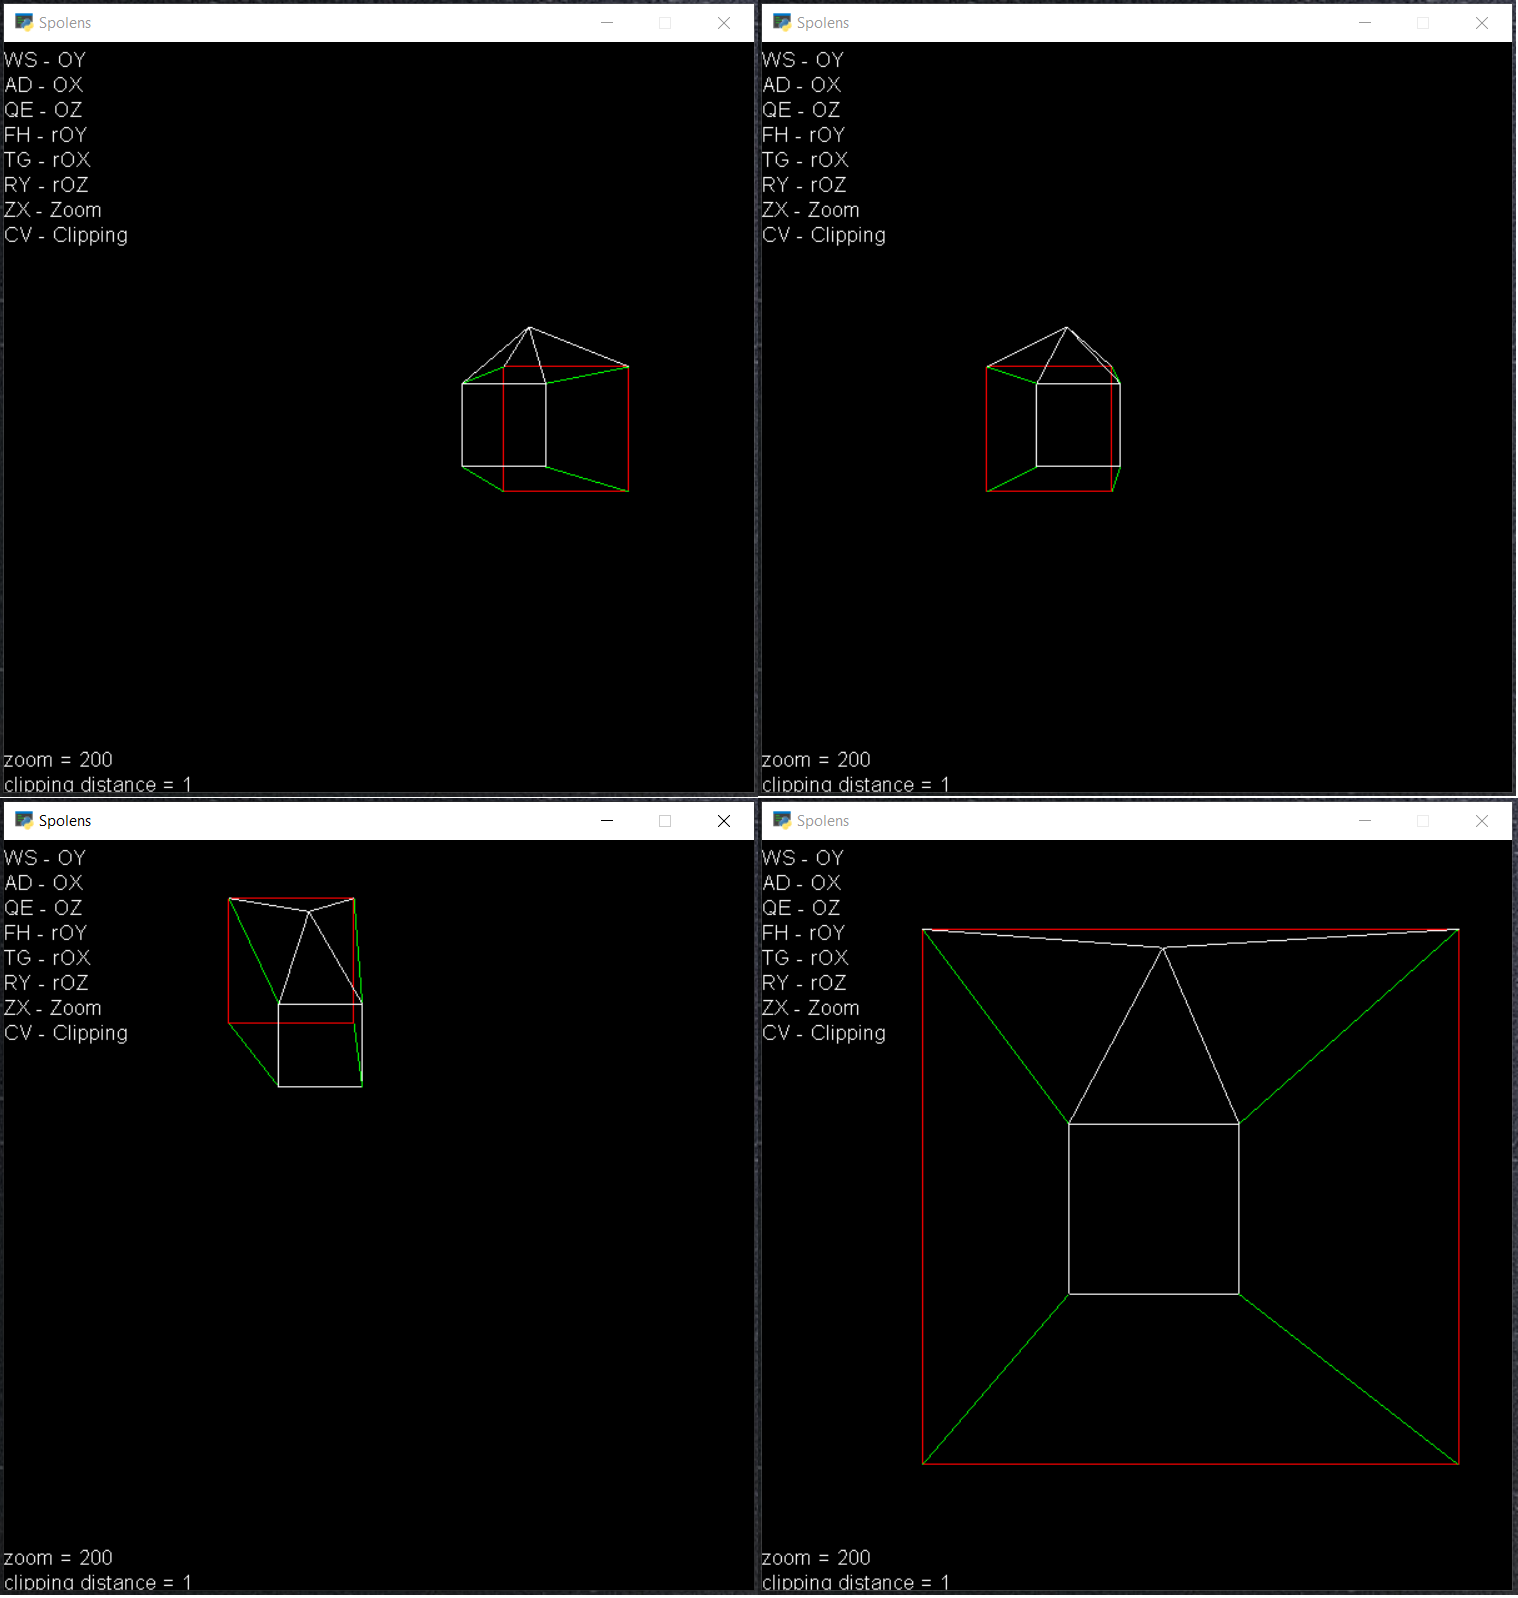
\includegraphics[scale=0.5]{spolens tra.png}
\end{center}

\newpage
\subsection{Rotacja}
Rotacją kontrolujemy za pomocą klawiszy:
\begin{itemize}
    \item F/H w osi OY,
    \item T/G w osi OX,
    \item R/Y w osi OZ.
\end{itemize}

\begin{center}
    \noindent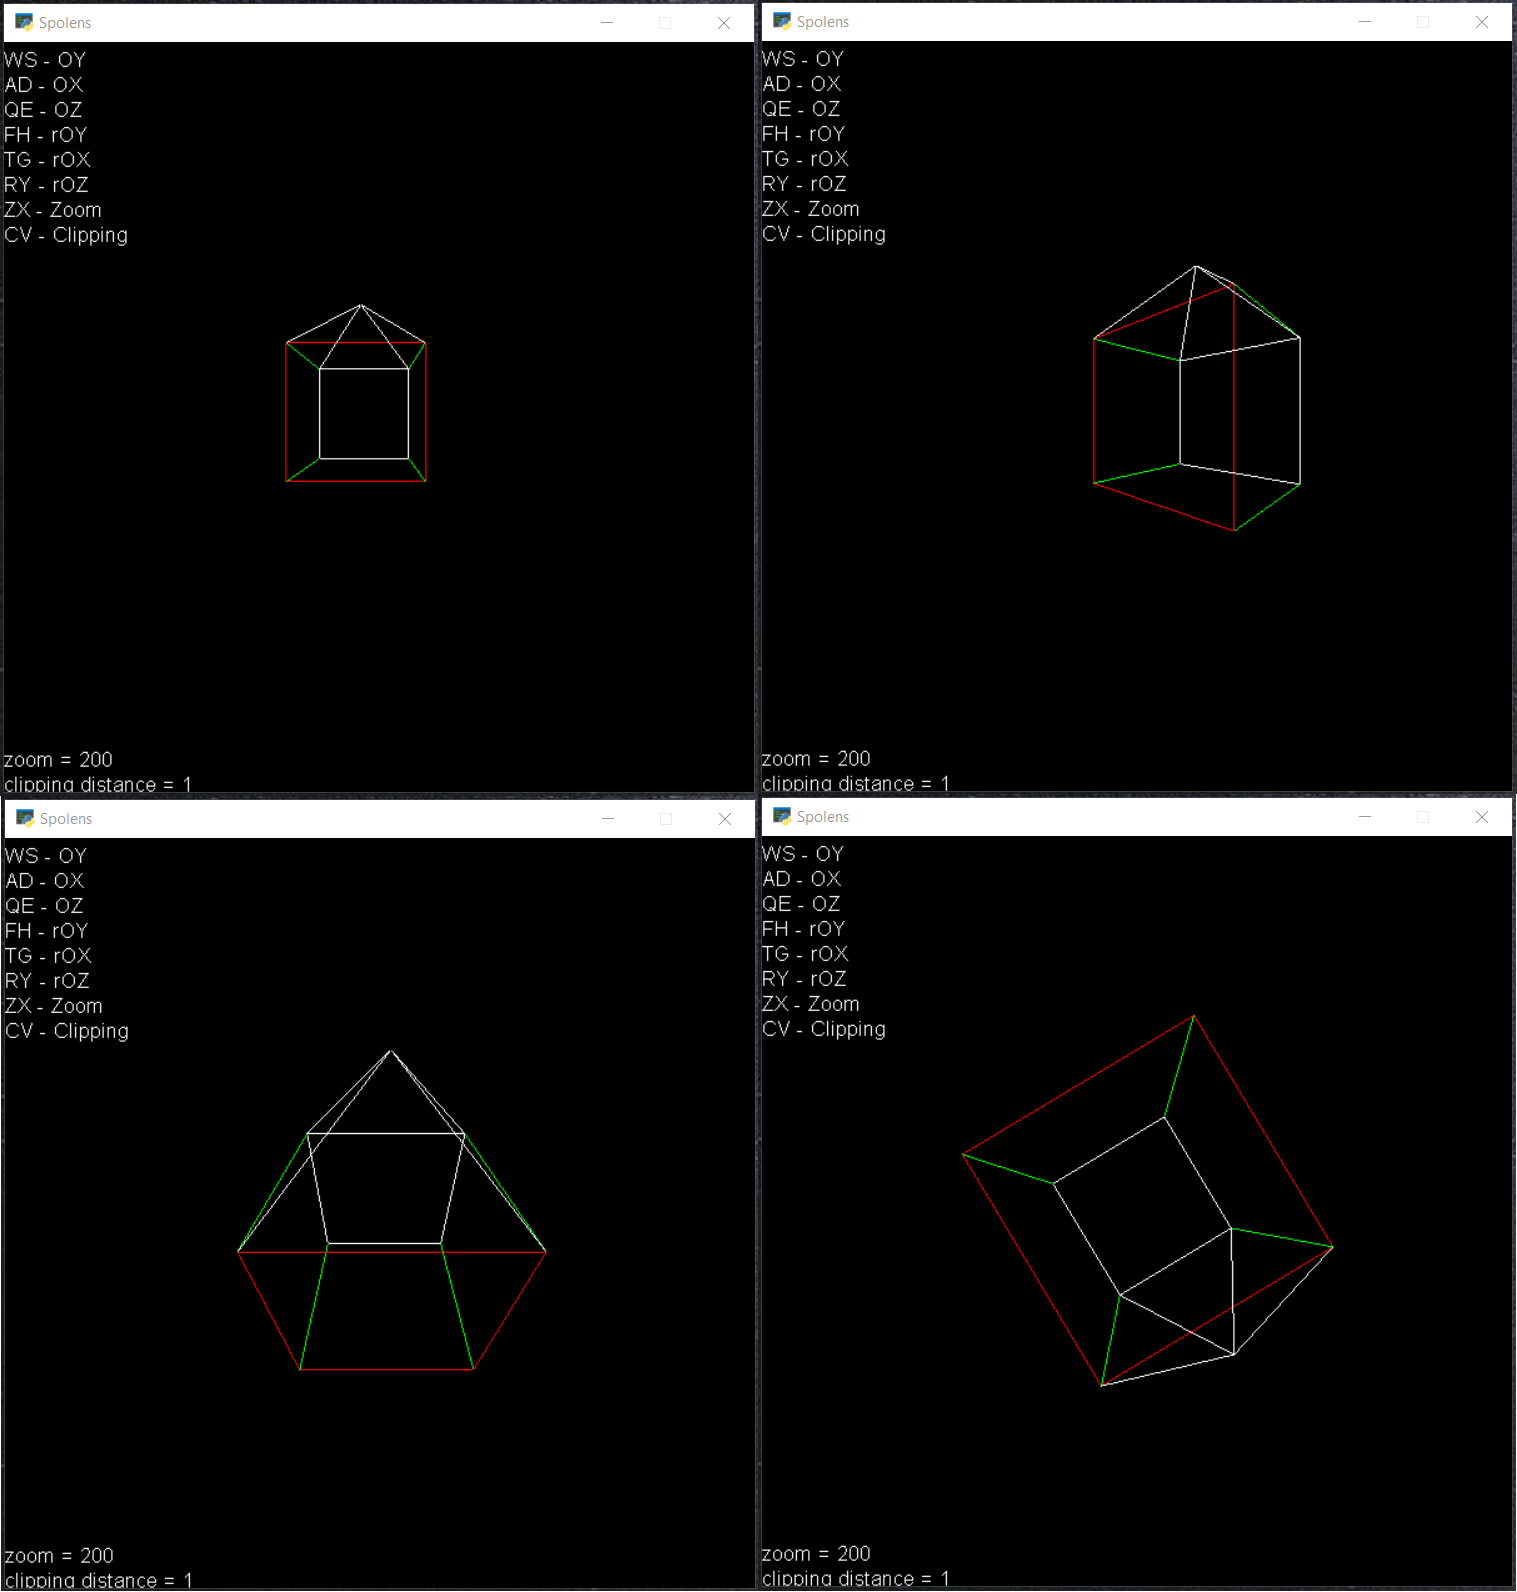
\includegraphics[scale=0.5]{spolens rot.png}
\end{center}

\newpage
\subsection{Zoom}
Przybliżeniem kontrolujemy za pomocą klawiszy Z/X. Dodatkowo informacja o wartości tego parametru jest wyświetlana w lewnym dolnym rogu. Jest to operacja różna od przesunięcia w osi OZ. Widać to po rozciągnięciu sześcianu.

\begin{center}
    \noindent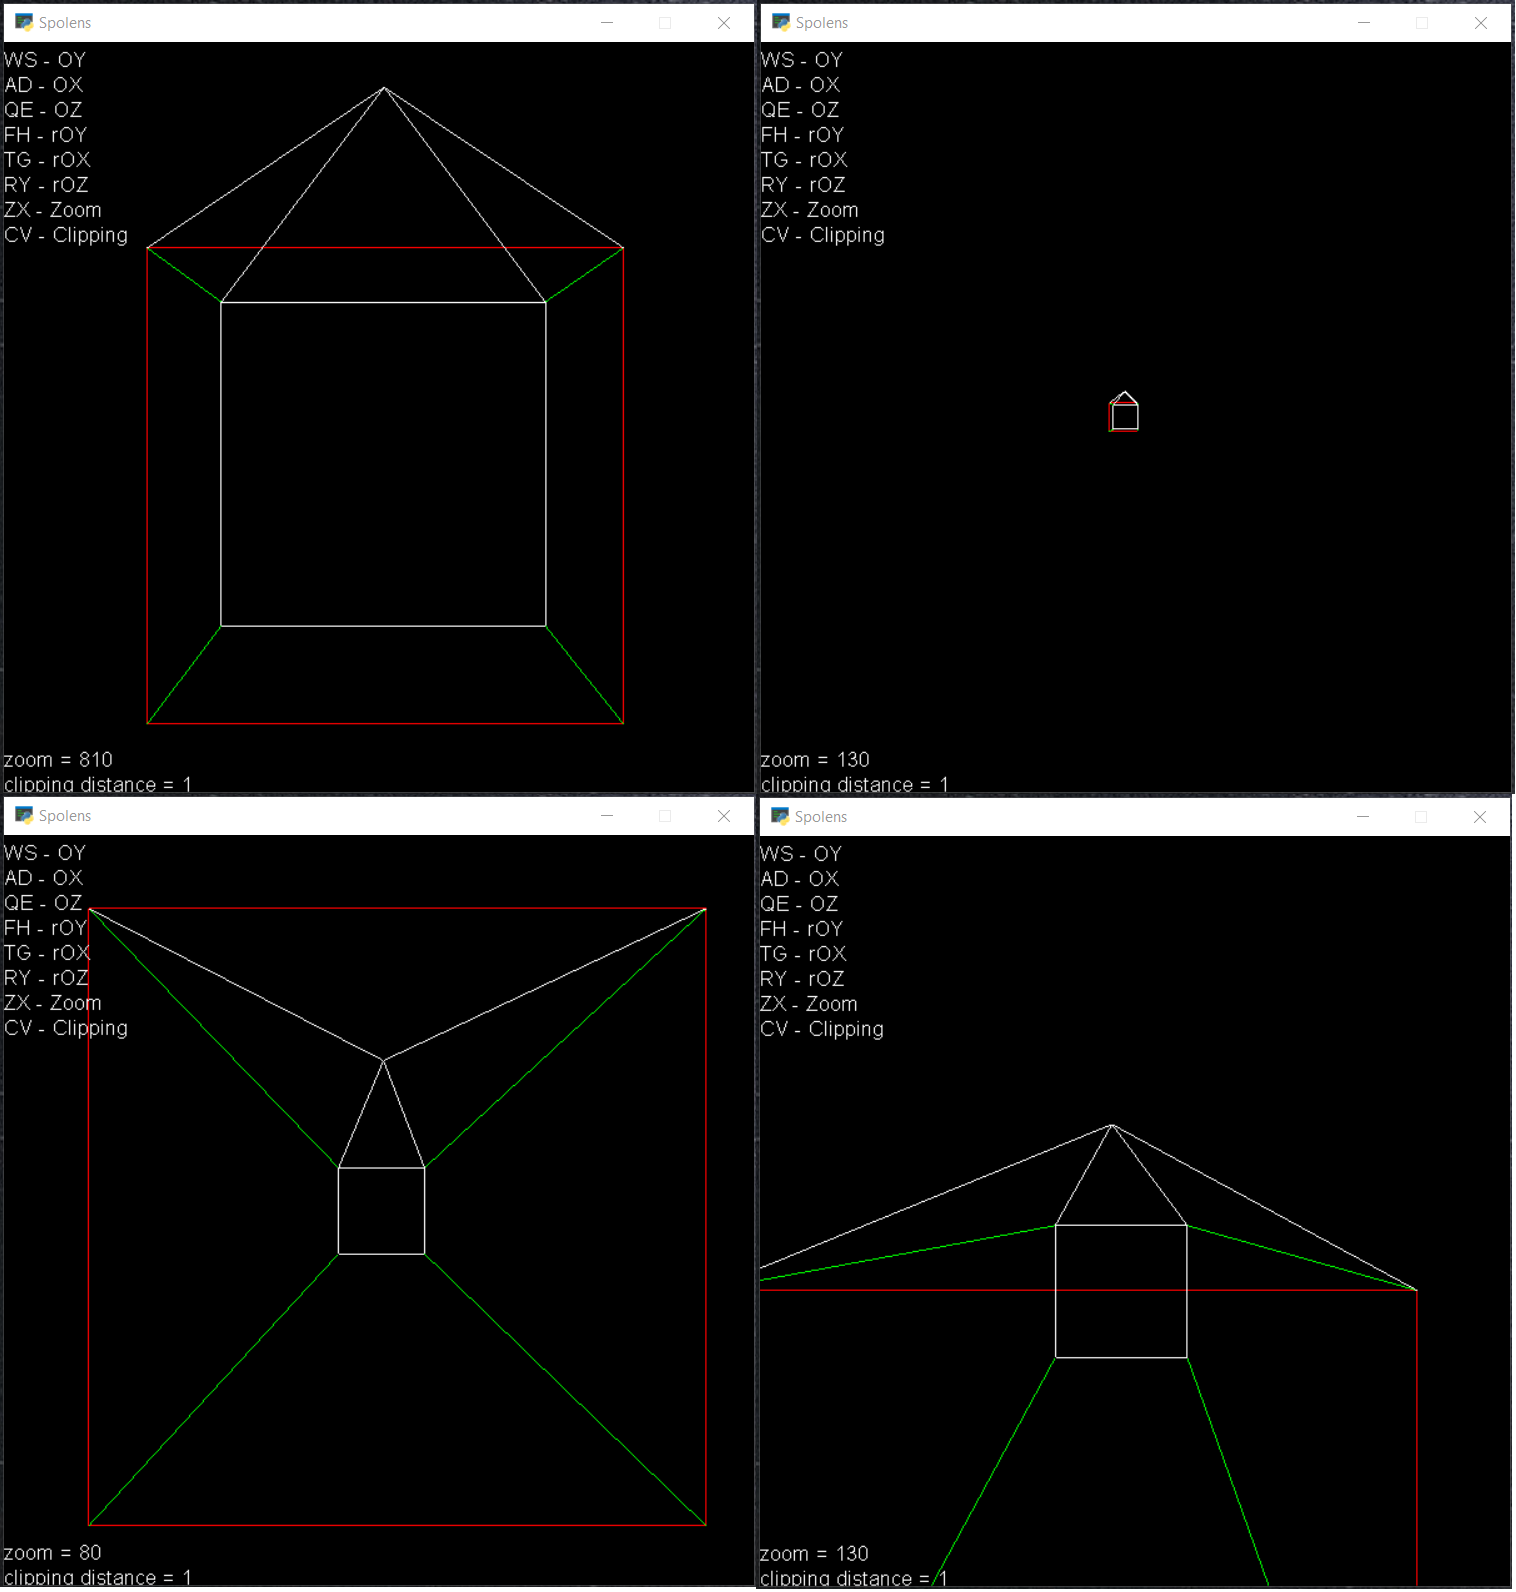
\includegraphics[scale=0.5]{spolens zoom.png}
\end{center}

\newpage
\subsection{Płaszczyzna ścinająca (Clipping Plane)}
Linie, które są za płaszczyzną ścinającą (kamerą), są ignorowane przy rysowaniu. Zaś linie które przechodzą przez tą płaszczyznę, są przycinane do punktu przecięcia się płaszczyzny z linią. Zapewnia to poprawne wyświetlanie obrazu w każdej pozycji kamery.

Płaszczyzną ścinającą (clipping plane) sterujemy klawiszami C/V, a wartość parametru jest wyświetlana w lewym dolnym rogu.

\begin{center}
    \noindent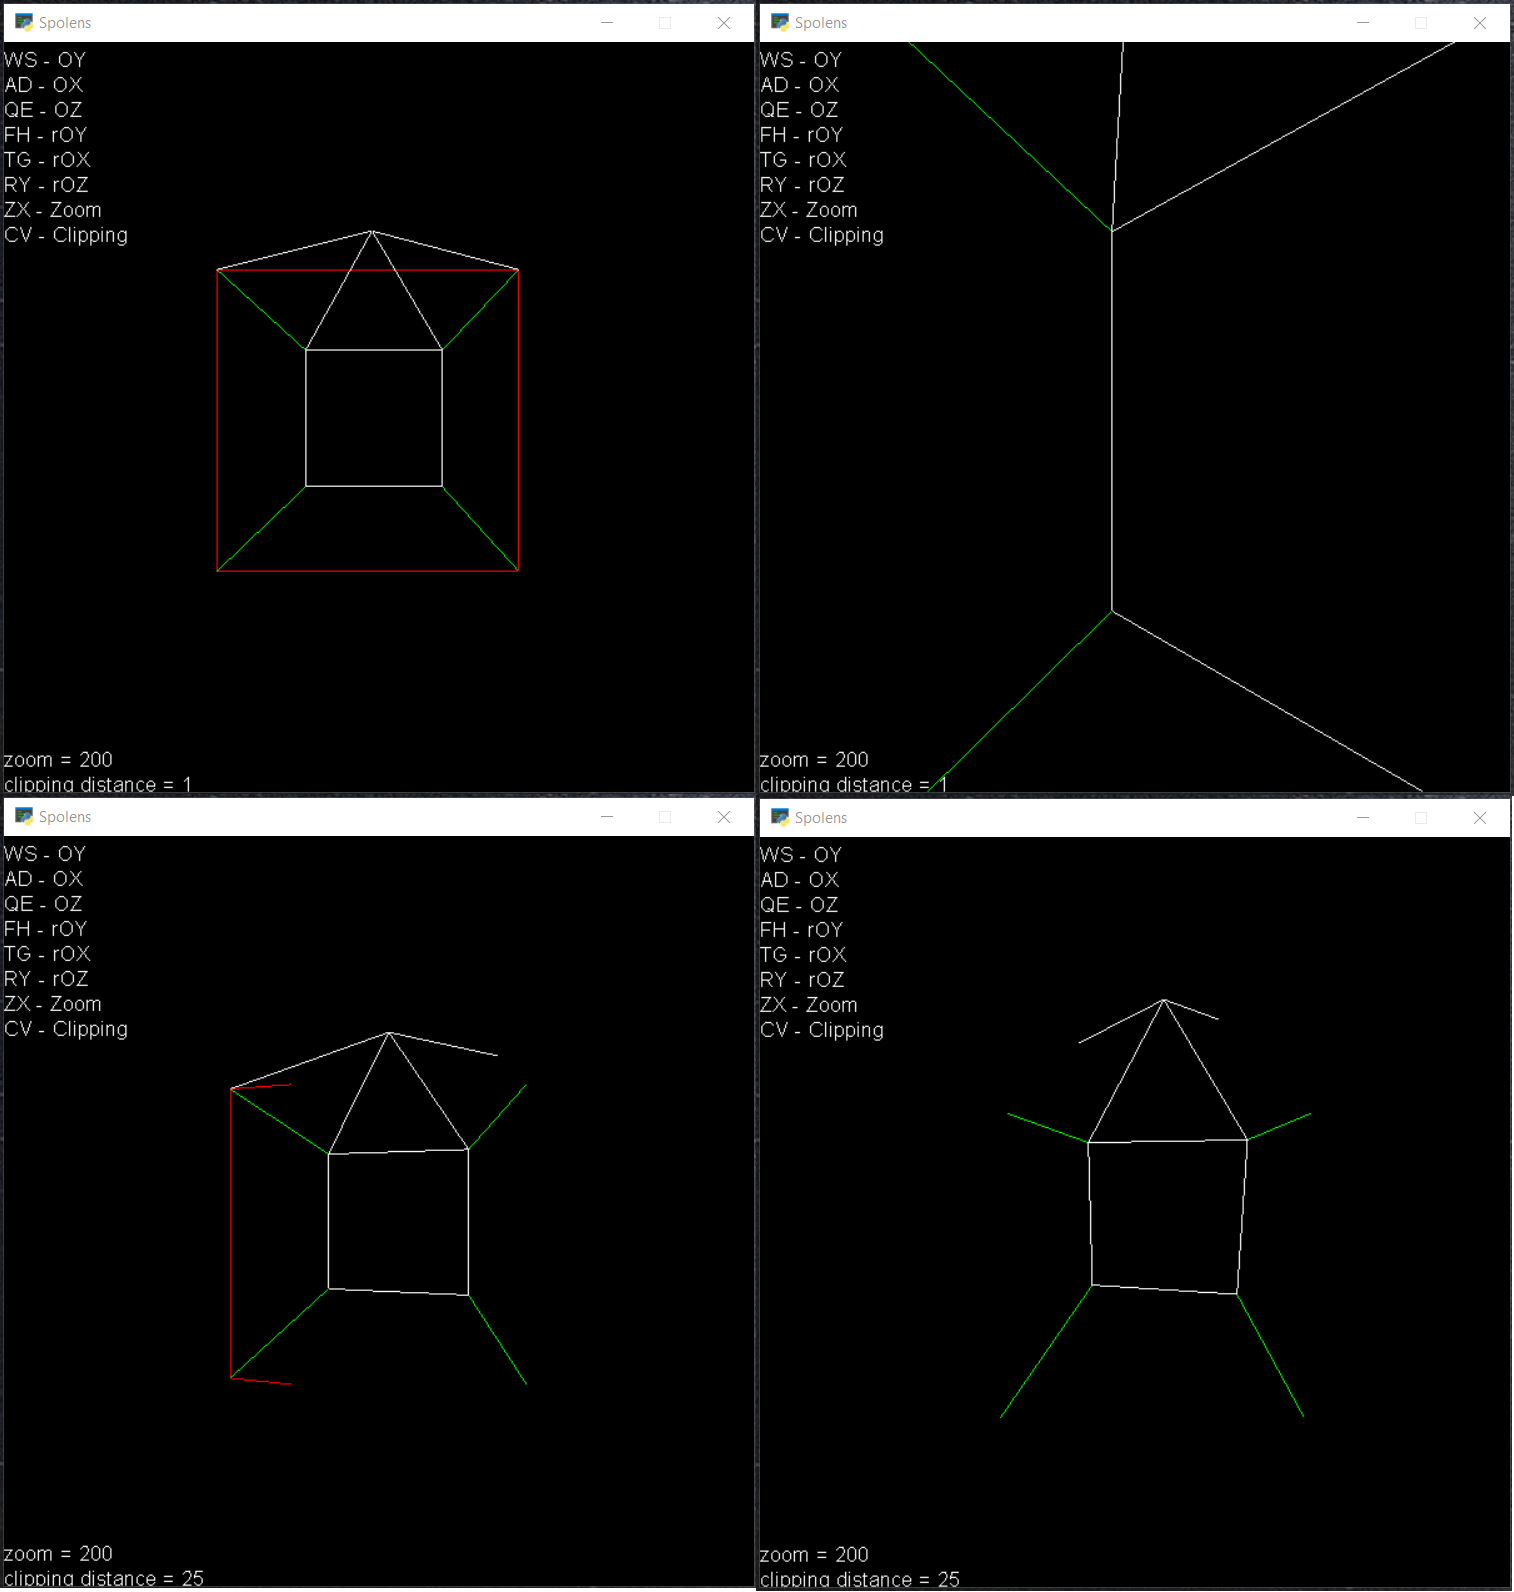
\includegraphics[scale=0.5]{spolens clip.png}
\end{center}

\newpage
\section{Struktura pliku konfiguracyjnego}
Plik w formacie .TXT składa się z linii w których ważny jest pierwszy znak, który określa typ danych jakie zawiera linia.

Tymi znakami są P i C, a linie które zaczynaja się z innym znakiem są ignorowane.

\subsection{Przykładowy plik konfiguracyjny}
\begin{lstlisting}[frame=single]  % Start your code-block

jakis komentarz

P frontDownLeft 30 30 60
P frontDownRight 60 30 60

C frontDownLeft frontDownRight 1 0 0 1

P top 45 75 75

C frontUpLeft top 1 1 1 1
\end{lstlisting}


\subsection{Linie zaczynające się od P}
Linie zaczynające się od P (od Point), definiują punkty i zawierają dane w formacie:
\begin{center}
    P [nazwa punktu] [x] [y] [z]
\end{center}

Gdzie: 
\begin{itemize}
    \item {[nazwa punktu]} to unikalny identyfikator punktu, którego należy używać przy definiowaniu połączeń (lini),
    \item {[x] [y] [z]} to parametry położenia punktu w przestrzeni trójwymiarowej.
\end{itemize}

\subsection{Linie zaczynajace się od C}
Linie zaczynajace się od C (od Connection), definiują połączenia pomiędzy punktami i zawierają dane w formacie:
\begin{center}
    C [nazwa punktu] [nazwa punktu2] [R] [G] [B] [A]
\end{center}

Gdzie: 
\begin{itemize}
    \item {[nazwa punktu]} i [nazwa punktu2] to ID punktów między którymi biegnie linia,
    \item {[R] [G] [B] [A]} to parametry koloru w formacie RGBA w przedziale wartosci od 0 do 1.
\end{itemize}

\end{document}